\documentclass[10pt]{article}

% Import packages
\usepackage{graphicx}
\usepackage{titling}
\usepackage{geometry}
\usepackage{subcaption}

\graphicspath{{./images/}}

\title{Lab 4 Report}
\author{Chad Lape and Colton Murray}
\date{Febuary 19th, 2020}

\begin{document}

	\maketitle
	
	\section{Objectives}
	This lab explored ideas of polymorphism and inheritence. This being that a base class was created which was inherited by two other derived classes which then had further implementation of its function play. This is very important to the field of Computer Science as this is the basis for object oriented programming and is often used extensively in the field. Polymorphism was found through the creation of a virtual function which was redefined in the derived classes and enabled it to have more than one functionality depending on how the class was called.
	
	\newpage
	\section{Task Documentation} 
	\subsection{Task 1}
	The show class had plenty of memebers, but only a few were going to be modified or usable by its derived classes. The available information was only the setters and getters of private information and the function play. Though by proxy of the setters and getters, the title and description are effectively public.
	\begin{itemize}
	\item [Public:]
		\begin{itemize}
			\item Setter/Getter
			\item Default Constructor
			\item Fill Constructor
			\item Play Function
		\end{itemize}
	\item [Private:]
		\begin{itemize}
			\item Title
			\item Description
		\end{itemize}
	\end{itemize}

	\subsection{Task 2}
	Description of the availability of TV Shows members to instances of itself and  declared as a base class.
	\begin{itemize}
		\item [TV Show]
		\begin{itemize}
			\item Derived Class Instance: 
			\begin{itemize}
				\item Full Functionality of all members
			\end{itemize}
			\item Base Class Instance: 
			\begin{itemize}
				\item Functionality of constructors
				\item Functionality of virtual play function
				\item Functionality of base class functions
				\item No Functionality from derived class functions
			\end{itemize}
		\end{itemize}
		\item[Movie]
		\begin{itemize}
			\item Derived Class Instance:
			\begin{itemize}
				\item Full Functionality of All Members
			\end{itemize}
			\item Bas Class Instance:
			\begin{itemize}
				\item Functionality of Constructors
				\item Functionality of virtual Play Function
				\item Functionality of Base Class Functions
				\item No Functionality of Derived Class Functions
			\end{itemize}
		\end{itemize}
	\end{itemize}
\newpage
	\subsection{Task 3}
	\begin{figure}
		\centering
		\begin{subfigure}{.8\textwidth}
			\centering
			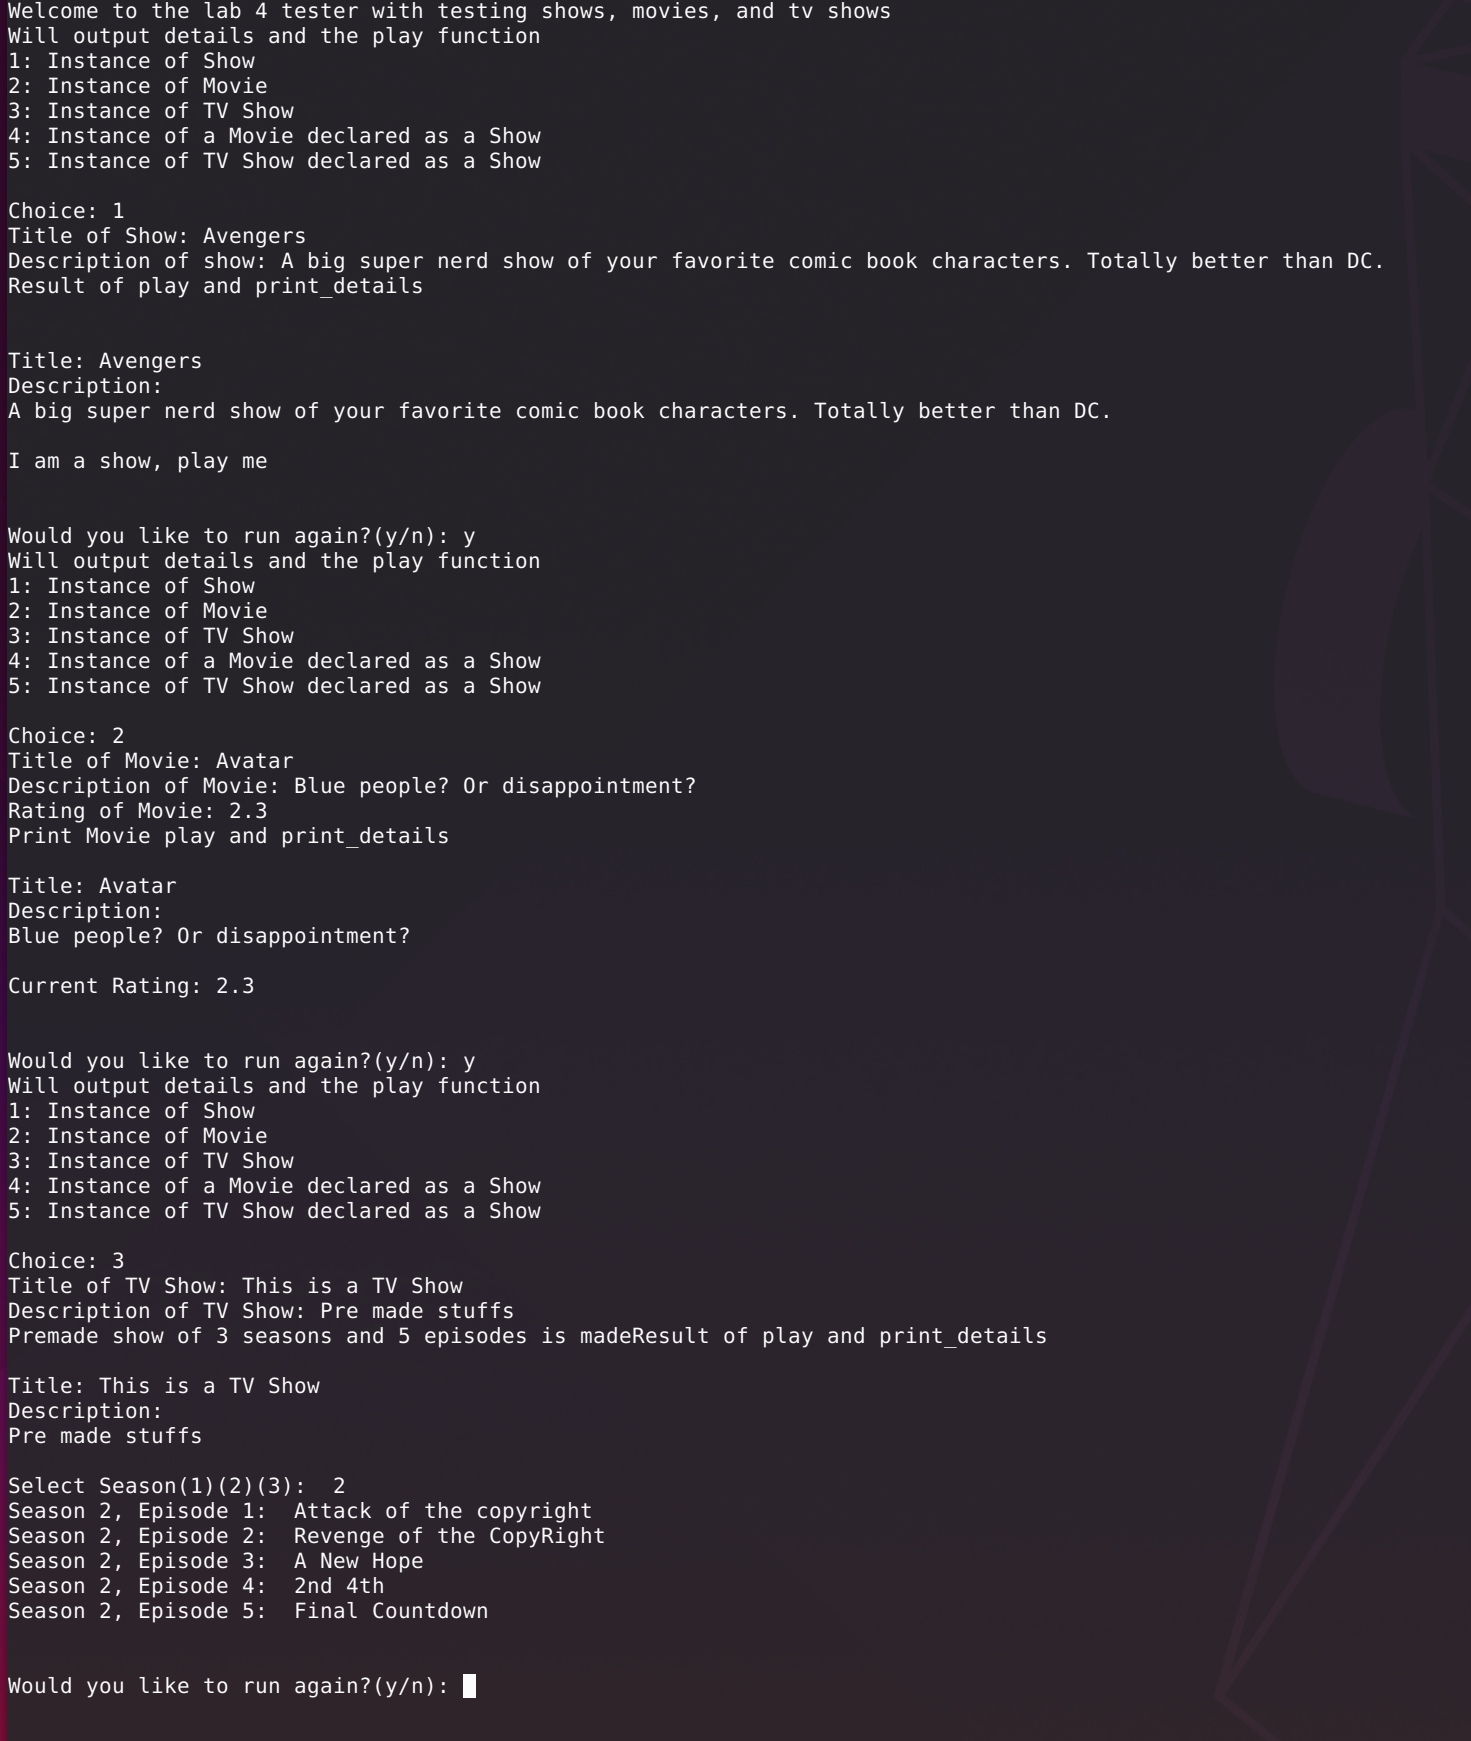
\includegraphics[width=0.7\linewidth]{Screenshot41}
		\end{subfigure}
		\begin{subfigure}{.8\textwidth}
			\centering
			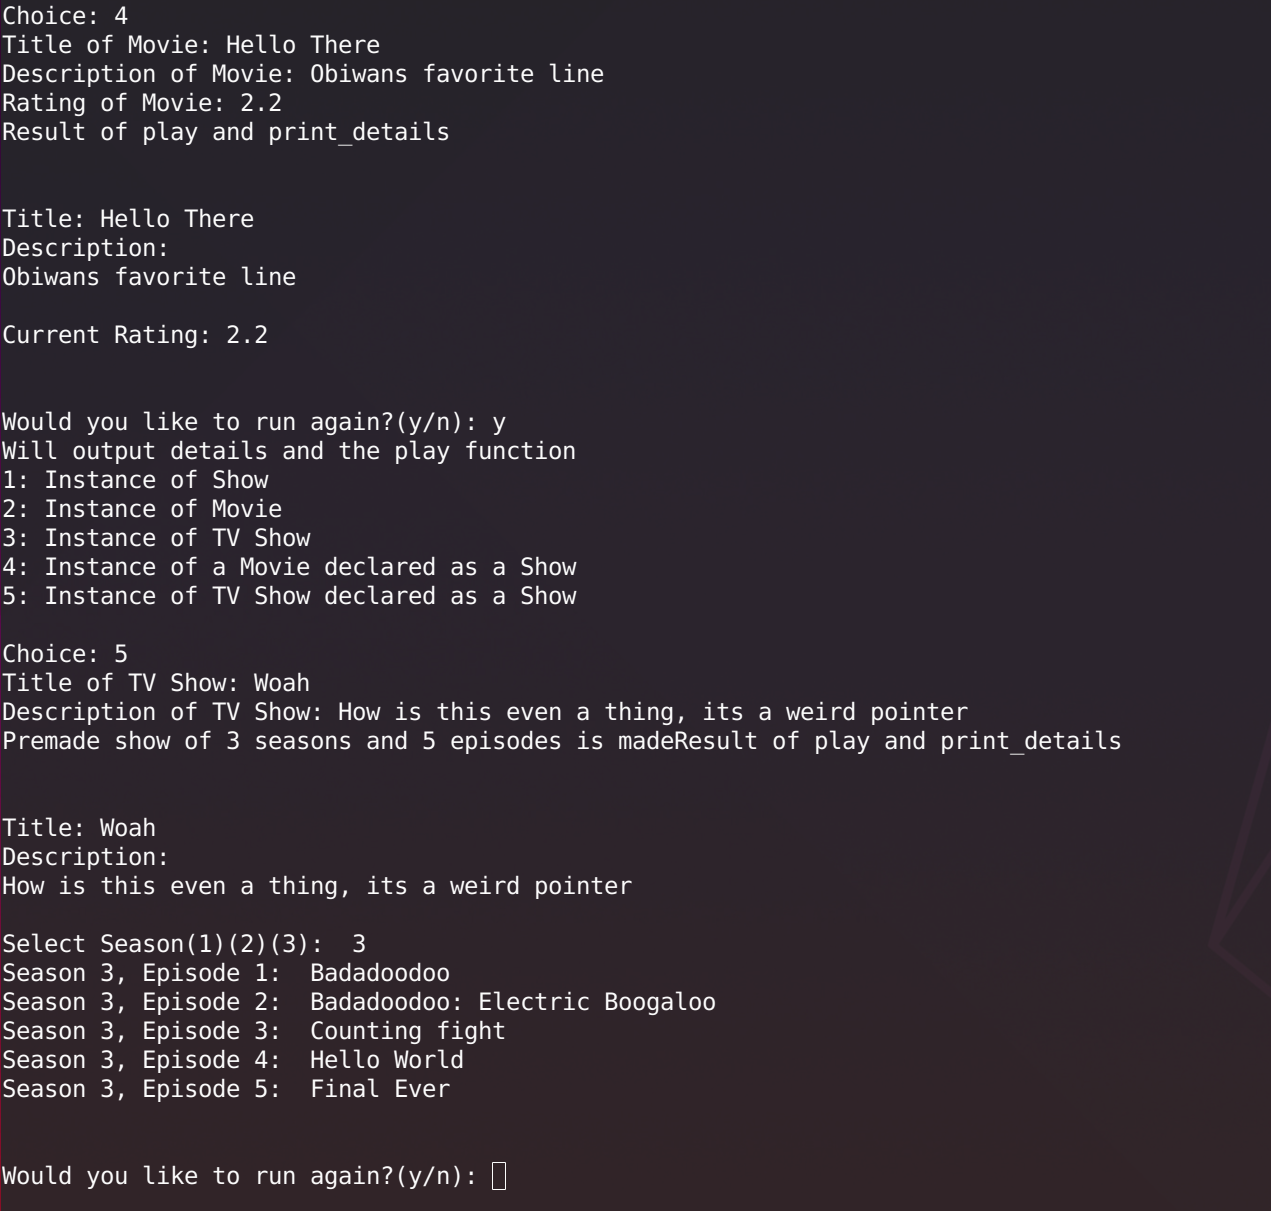
\includegraphics[width=0.7\linewidth]{Screenshot42}
		\end{subfigure}
	\caption{Screenshots}
	\end{figure}
	\begin{itemize}
		\item [Results]
		The Results worked as expected. Due to the pointers calling new derived object constructors, this enabled the information within the derived class to be accessed by the base class. Additionally, the base class pointer was able to access the virtual function which allowed for a polymorphism to occur.
	\end{itemize}
	\section{Contribution}
	All members in the team had worked together on creating the different parts, what follows is to have some extra context.
	\begin{itemize}
		\item [Chad:]
		\begin{itemize}
			\item Created base Show Class
			\item Created Movie Class
			\item Made tester for both
			\item Created Lab Report
		\end{itemize}
		\item[Colton:]
		\begin{itemize}
			\item Created TV Show Class
			\item Created tester for TV Show
			\item Created way to interact with 2d array of episodes
		\end{itemize}
	\end{itemize}
	\subsection{Compiling}
	Use pre compiled version of lab4.exe. Take that and use the sources which are included to be seen. Use mingw to compile or insert the sources into a visual studio project to compile.

\end{document}